%第13章,功能
\chapter{功与能}
\label{Work and Energy}
微小至微观粒子的亲和,宏大到恒星的湮灭,能量与这些这些过程中息息相关。一个人的能量太过渺小。但是恒河沙数般的人类集合也能够带来伟大的改变。

\begin{TaskBox}
这句话当中的两处能量一处是物理意义上的,还有一处是文学意义上的。这两个的定义并不相同。思考一下两者的区别。
\end{TaskBox}

\section*{学习目标}
\begin{todolist}
 \item 理解力可以做功,并求算恒力做功
 \item 理解能量的概念,掌握动能和重力势能的求算
 \item 理解能量变化与外力做功的关系
 \item 掌握并使用能量守恒定理
 \item 理解功率的意义
 \item 求算包含阻力做功的情况
\end{todolist}
\clearpage


\section{做功}
\label{sec:Work done}

\gls{work}被定义为力与位移的点乘。单位为\si{\J}
\[
	W=\vec{F}\cdot \vec{s}=|\vec{F}||\vec{s}|\cdot \cos{\theta}
\]
如下图所示,在一个物体运动过程中,力所做出的功为
\begin{figure}[H]
\centering
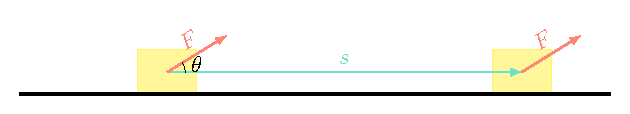
\includegraphics[width=0.8\textwidth]{workdone}
\caption{在整个过程中,力的大小和方向是不变的}
\end{figure}

\begin{TaskBox}
根据做功的定义,尝试把\si{\J}表示为国际制基础单位。
\tcblower
思考一下,做功是一个标量还是矢量,是一个过程量还是一个状态量
\end{TaskBox}
\clearpage

\section{能量}
\label{sec:Energy}
一个物体或者系统所具有的能量可以理解为该物体能够对外界做功的能力大小。因此从这个角度上来说能量和做功是息息相关的。在A Level数学部分中能量章节中,掌握重力势能和动能就可以了

\subsection*{重力势能}
\label{subsec:Gravitational Potential Energy}
\gls{gpe}顾名思义就是与重力有关的能量,当一个物体处于更高的高度的时候,该物体会具有更多的重力势能;即使在同样的高度处,质量更大的物体重力势能更多。如下图所示
\begin{figure}[H]
\centering
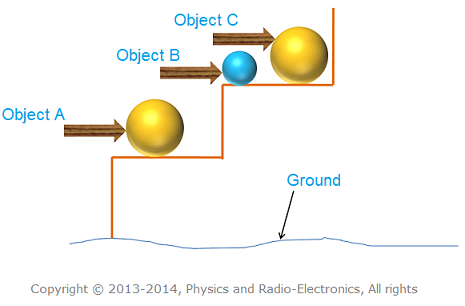
\includegraphics[width=0.8\textwidth]{gpe} 
\caption{重力势能与高度和物体质量有关系}
\end{figure}

因此重力势能的定义公式为:
\[
	GPE=mgh_{_{relative}}
\]
这里的$h_{_{relative}}$是一个瞬时状态量,指求算重力势能的物体的质心到规定的\gls{reflevl}的高度,且如果低于\gls{reflevl}则认为重力势能为负值。这里的负号与速度或者加速度的符号含义不一致,不代表方向。仅代表该能量小于0。

\subsection*{动能}
\label{subsec:Kinetic Energy}
当物体处于运动状态的时候,该物体就具有了\gls{ke}。通过定性地分析,不难发现一个物体运动速度越快,动能必定越大;即使两个物体具有同样的速度,质量更大的物体,动能越大。所以动能的大小求算则被定义为:
\[
	KE=\frac{1}{2}mv^2
\]
\begin{figure}[H]
\centering
\includegraphics[width=0.8\textwidth]{ke}  %图像还没有找
\caption{动能的大小和质量以及速度有关}
\end{figure}
\clearpage

\section{能量守恒}
\begin{TaskBox}
 推导动能和重力势能的国际制单位
\end{TaskBox}
功和能量的单位是一样的,这两个物理量必定是互相相关联。

\subsection*{功能关系}
一个系统的能量如果发生的变化,必定是由于外力持续做功了。是非常著名的\textbf{work-energy principle},其描述如下:
\begin{theorem}
Increase in kinetic energy = total work done by all forces
\end{theorem}
写成公式的形式为:
\[
	\Delta KE = \sum Fs
\]
其中,有些力做正功,能够增加系统的动能,有些力做负功,会降低动能,我们所说的total work done是指这些正功与负功的全部累积。

\subsection*{机械能守恒定律}
\subsubsection*{保守力与势能}
\gls{consforce}做功与路径无关,并且,保守力做过的功会与系统的势能息息相关。

\begin{ExampleBox}
求算质量为$1$\si{\kg}的铁球,下落$5$ \si{\m}的过程中,重力做功,以及重力势能的变化量
\tcblower
(i) 重力竖直向下,下落的位移也是竖直向下的, 因此重力做正功,根据做功的求算
\begin{align*}
	W &= F\cdot s\\
	  &=mg \cdot h\\
	  &=1\times 10 \times 5\\
	  &=50 \si{\J}
\end{align*}

(ii) 假设下落开始的时候作为参考面,重力势能为0;末状态铁球的高度在$-5$ \si{\m}的地方。因此末状态的重力势能为:
\[
	GPE_f = mgh =1\times 10\times (-5) = -50\si{\J}
\]
所以,重力势能的变化量为:
\[
	\Delta GPE = GPE_f-GPE_i =-50-0 =-50\si{\J}
\]
\end{ExampleBox}
在上面的例子中,重力势能的求算和重力做功的求算公式几乎是一致的,但是细品一下,在重力做功求算中,$5$\si{\m}是一个过程量,是下落的位移;在重力势能的求算过程中$-5$\si{\m}是一个状态量,是下落过程末状态的高度。但是初状态的高度减去末状态的高度就是下落的位移。因此重力势能的变化量,与重力所做的功是大小相等的,但是方向相反。

因此对于重力势能和重力做功而言,始终有这样的关系:
\[
	W_{con} =-\Delta GPE
\]
而这个关系对于其他的势能也是成立的。只不过不要局限于重力势能。

\subsubsection*{机械能守恒的条件}
机械能就是物体的动能和势能之和。当一个系统中,做功的力是保守力的时候,我们可以把work-energy principle以及势能和保守力的关系联合在一起进行如下的推导:

\begin{align*}
  \Delta KE  &= \sum W =W_{con} = -\Delta PE\\
  \Delta KE  &=-\Delta PE\\
  \Delta KE +\Delta PE &=0\\
  KE_i+PE_i &= KE_f+PE_f
\end{align*}

因此,这就是机械能守恒定律:
\begin{theorem}
 When gravity (conservative force) is the only force which does work on a body, mechanical energy is conserved for the whole process
\end{theorem}


\begin{ExampleBox}
The diagram shows a wire $ABCD$ consisting of a straight part $AB$ of length $5$ \si{\m} and a part $BCD$ in the shape of a semicircle of radius $6$ \si{\m} and centre $O$. The diameter $BD$ of the semicircle is horizontal and $AB$ is vertical. A small ring is threaded onto the wire and slides along the wire. The ring starts from rest at $A$. The part $AB$ of the wire is rough, and the ring accelerates at a constant rate of $2.5$ \si{\m \per\square \s}  between $A$ and $B$.As it reaches $B$, the speed is $5$ \si{\m\per\s}.The part $BCD$ of the wire is smooth. The mass of the ring is $0.2$ \si{\kg}.
\begin{figure}[H]
\centering
\includegraphics[width=0.3\textwidth]{semicircle}
\end{figure}
Find the speed of the ring at $C$, where angle $BOC$ = $30$ \si{\degree}.\\
\makebox{}\hfill Adapted from $2017$ summer qp $42$ $Q2$

\tcblower
当珠子沿着BC段下滑时,由于光滑无摩擦,并且支持力不做功,只有重力做功,因此满足机械能守恒定律。\\
$PE \ loss = mgr\cdot \sin 30=0.6\times 10 \times 6 \times \sin 30=18\si{\J}$\\
$KE \ gain =\frac{1}{2}m(v_C^2-v_B^2)$\\
因为$PE \ loss=KE \ gain$, 所以求算出$v_C=9.22\si{\m\per\s}$
\end{ExampleBox}

\begin{figure}[H]
\centering
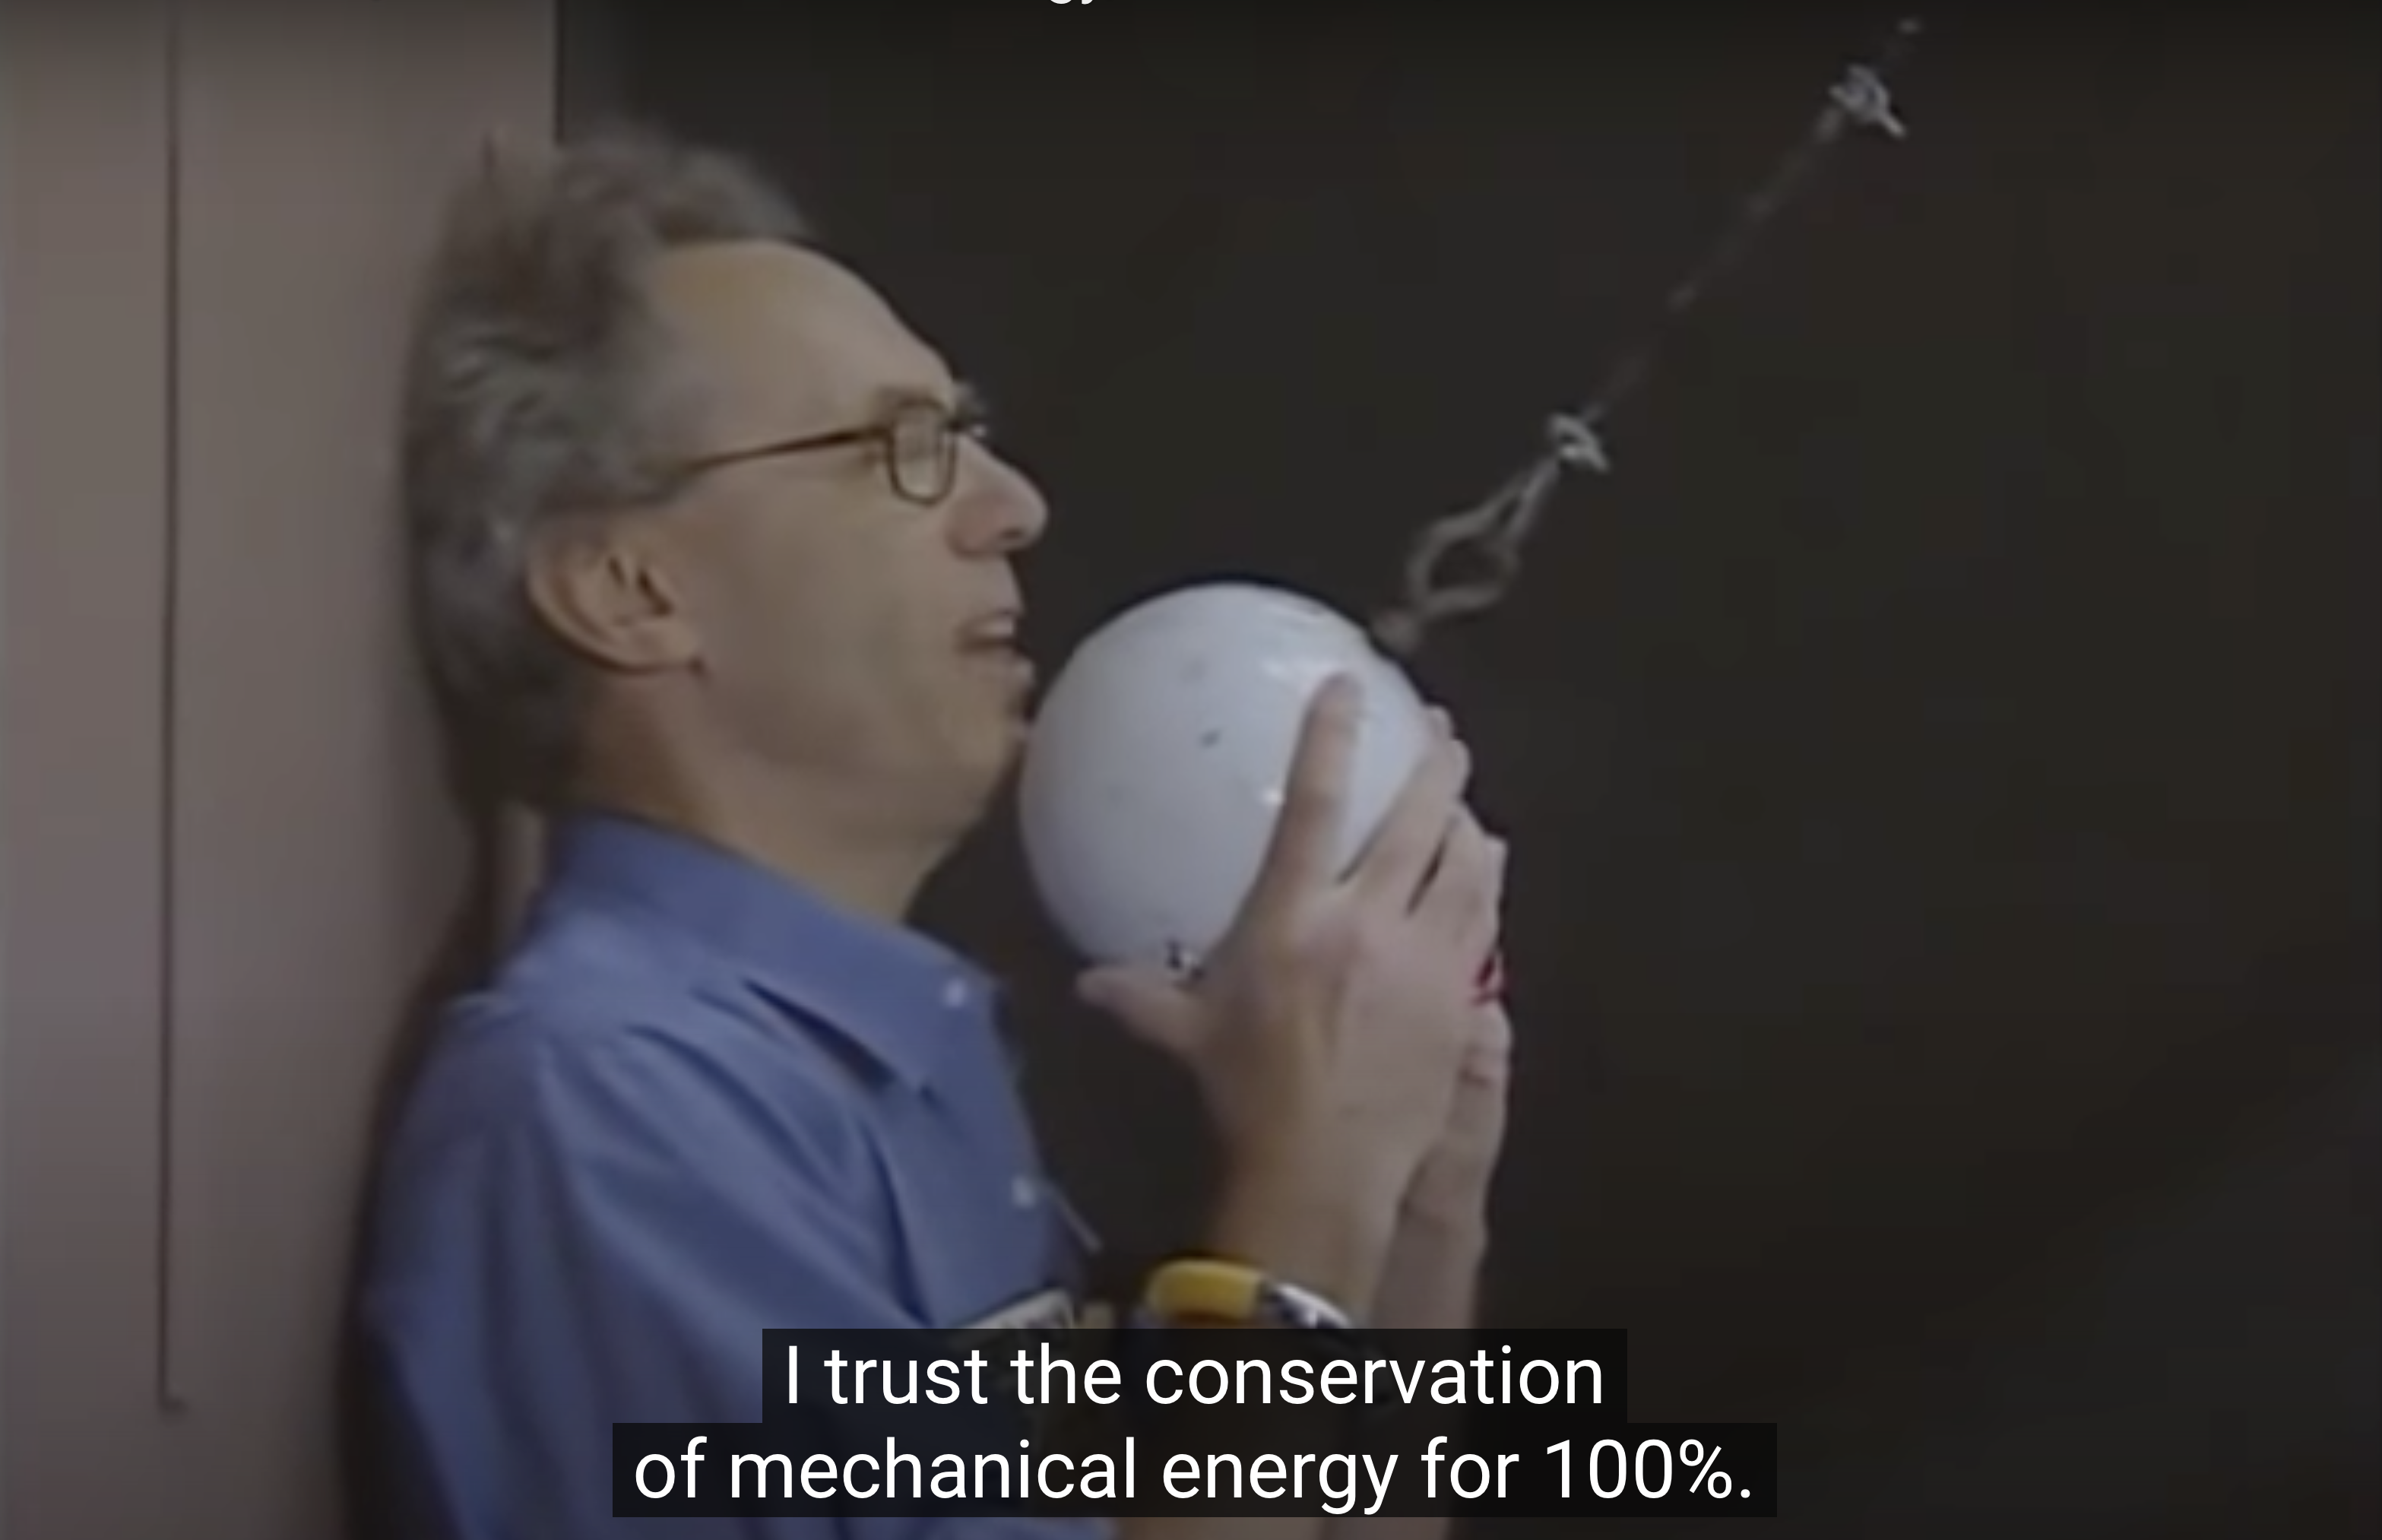
\includegraphics[width=0.8\textwidth]{conservation}
\caption{教授说相信守恒定律}
\end{figure}

\begin{TaskBox}
教授从静止释放小球可以安全存活,要怎么样作死才会使小球回来的时候打到下巴。这个时候的机械能还守恒吗?如果守恒的话该怎么样列表达式
\end{TaskBox}

\subsection*{能量守恒定律}
当然机械能守恒能够发生还是需要满足一定要求的,但是下面这种守恒则是完美地通用地适合于一切场景,它就是守恒律中的一颗明珠:标题已经剧透了。
\begin{theorem}
 Energy cannot be created or destroyed. It can only be converted from one form to another.
\end{theorem}

那我们之前不是说外力做功可以或者减少系统的能量吗?那不是和能量守恒定律相违背了吗?其实没有,因为外力做功也是需要消耗能量的。总体的能量依旧守恒,保持不变。比如推箱子
\begin{figure}[H]
\centering
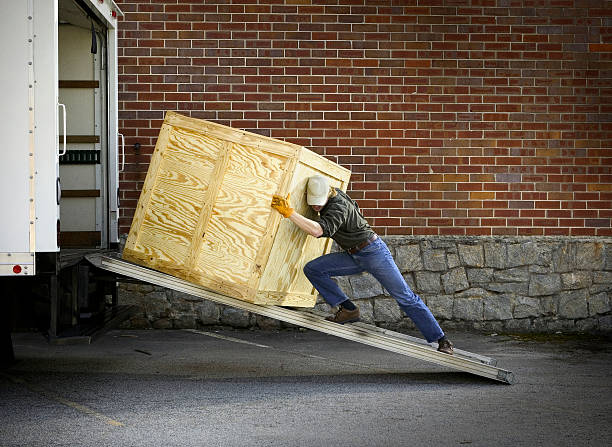
\includegraphics[width=0.8\textwidth]{pushbox}
\caption{匀速前进的箱子}
\end{figure}
人的推力对箱子做了正功,但是这个正功的来源是人身体内的化学能。地面的摩擦力做了负功,但是这个减少的能量没有消失,而是转化成了热能。因此无论推箱子前还是推箱子后,人-箱子-地面构成的完整系统能量是守恒的。
\clearpage

\section{功率}
\gls{power}是描述物体做功快慢的物理量,单位为\si{\W}。因此,功率被定义为:
\begin{definition}
The rate of doing work\\
\[
	P=\frac{\text{work done by force}}{\text{time taken}}
\]
\end{definition}

\begin{TaskBox}
推导功率的SI基础单位
\tcblower
了解一下\href{https://mp.weixin.qq.com/s/tpszxZu7VZMLdc4Gpit49A}{瓦特}改良蒸汽机的历史,以及马力的定义
\end{TaskBox}

因此平均功率就是总功除以总的时间,而瞬时功率的求算则要通过 
\[
	P=\frac{\d W}{\d t}=F\cdot \frac{\d s}{\d t}=Fv
\]
进行求算。


\begin{ExampleBox}
A train of mass $240,000$ \si{\kg} travels up a slope inclined at an angle of $4$ \si{\degree} to the horizontal. There is a constant resistance of magnitude $18,000$ \si{\N} acting on the train. At an instant when the speed of the train is $15$ \si{\m\per\s} its deceleration is $0.2$ \si{\m\per\square\s} . Find the power of the engine of the train.\\
\makebox{}\hfill Adapted from $2018$ summer $qp42$ $Q2$

\tcblower
首先根据牛顿第二定律求算引擎提供的作用力
\begin{align*}
F_{engine}-mg\cdot\sin\theta - F_{resist} &=ma\\
F_{engine}-240000 \times 10 \times \sin 4-18000 &=240000\times (-0.2)
\end{align*}
得到 $F_{engine}=137,415.53$\si{\N}\\
然后利用瞬时功率的公式$P=Fv=137,415.53\times 15 =2,060,000$\si{\watt}
\end{ExampleBox}